\documentclass[12pt, a4paper]{article}

\usepackage{amssymb}
\usepackage{multicol}
\usepackage{enumerate}
\usepackage[top=5em, bottom=5em, left=5em, right=5em]{geometry}
\usepackage{listings}
\usepackage{tikz}
\usetikzlibrary{positioning}

\setlength\parskip{1em}
\setlength\parindent{0em}

\title{Assignment}

\author{Hendrik Werner s4549775}

\begin{document}
\maketitle

This was done in collaboration with Constantin Blach (s4329872).

\section{} %1
Initial state:

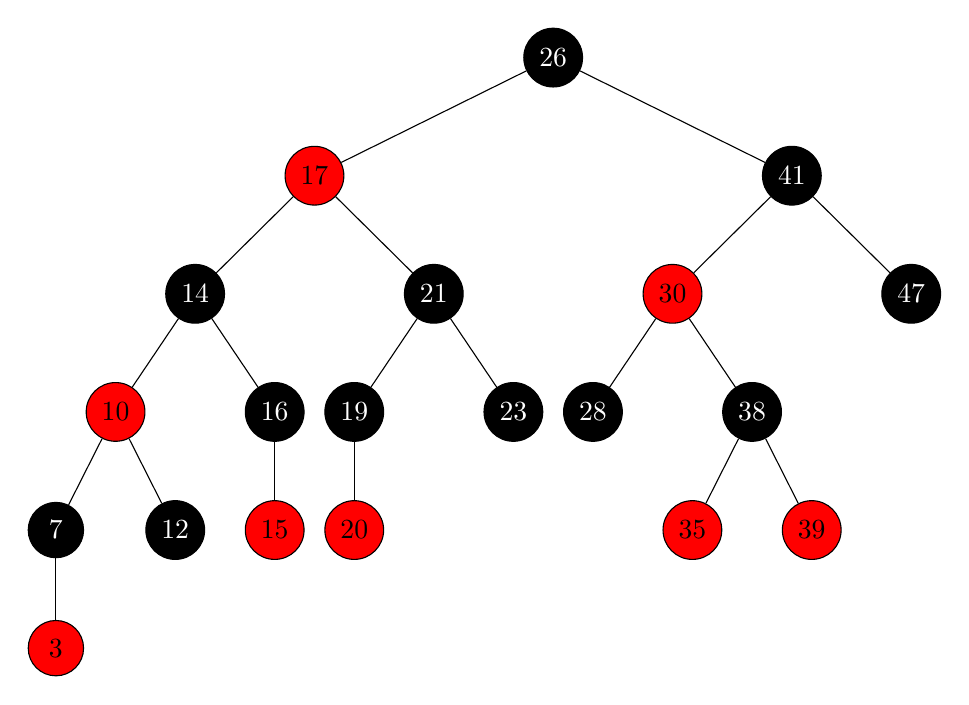
\begin{tikzpicture}[
	every node/.append style={minimum width=2em}
	,level/.style={sibling distance=.5\linewidth/#1}
	,b/.style={circle, draw, fill=black, text=white}
	,r/.style={circle, draw, fill=red}
]
	\node [b] (A) {26}
		child {
			node [r] (B) {17}
			child {
				node [b] (D) {14}
				child {
					node [r] (H) {10}
					child {
						node [b] (N) {7}
						child {
							node [r] (T) {3}
						}
					}
					child {
						node [b] (O) {12}
					}
				}
				child {
					node [b] (I) {16}
					child {
						node [r] (P) {15}
					}
				}
			}
			child {
				node [b] (E) {21}
				child {
					node [b] (J) {19}
					child {
						node [r] (Q) {20}
					}
				}
				child {
					node [b] (K) {23}
				}
			}
		}
		child {
			node [b] (C) {41}
			child {
				node [r] (F) {30}
				child {
					node [b] (L) {28}
				}
				child {
					node [b] (M) {38}
					child {
						node [r] (R) {35}
					}
					child {
						node [r] (S) {39}
					}
				}
			}
			child {
				node [b] (G) {47}
			}
		}
	;
\end{tikzpicture}

When adding the key 36 it is inserted at the following position:

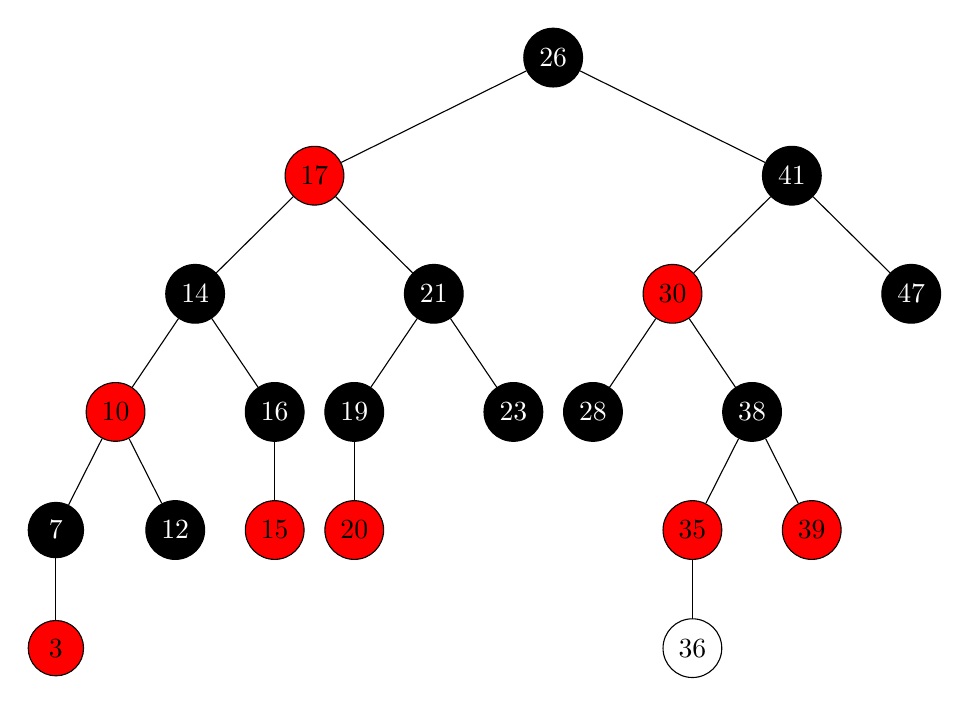
\begin{tikzpicture}[
	every node/.append style={minimum width=2em}
	,level/.style={sibling distance=.5\linewidth/#1}
	,b/.style={circle, draw, fill=black, text=white}
	,r/.style={circle, draw, fill=red}
]
	\node [b] (A) {26}
		child {
			node [r] (B) {17}
			child {
				node [b] (D) {14}
				child {
					node [r] (H) {10}
					child {
						node [b] (N) {7}
						child {
							node [r] (T) {3}
						}
					}
					child {
						node [b] (O) {12}
					}
				}
				child {
					node [b] (I) {16}
					child {
						node [r] (P) {15}
					}
				}
			}
			child {
				node [b] (E) {21}
				child {
					node [b] (J) {19}
					child {
						node [r] (Q) {20}
					}
				}
				child {
					node [b] (K) {23}
				}
			}
		}
		child {
			node [b] (C) {41}
			child {
				node [r] (F) {30}
				child {
					node [b] (L) {28}
				}
				child {
					node [b] (M) {38}
					child {
						node [r] (R) {35}
						child {
							node [circle, draw] (U) {36}
						}
					}
					child {
						node [r] (S) {39}
					}
				}
			}
			child {
				node [b] (G) {47}
			}
		}
	;
\end{tikzpicture}

We could either color it black, which would violate property 5 ("For each node, all paths from node to descendant leaves contain same number of black nodes"): The path $38 \rightarrow 39 \rightarrow nil$ has a black heigth of 1 while $38 \rightarrow 35 \rightarrow 36 \rightarrow nil$ has a black height of 2.

Alternatively we could color it red which would violate property 4 ("If a node is red, then both its children are black.") because 36 is a child of 35 and 35 is red.

\section{} %2

The maximum height of a red-black tree is $2bh$, where $bh$ is the black height of the root node. Thus the maximum height of a red-black tree with $bh = k$ is $2k$. The leaf node $nil$ is always present so we need to add it as well, and subtract one from the exponent because the leaf node exists only once.

We can calculate the maximum number of nodes which is $2^{2k - 1} + 1$.

\section{} %3

\begin{description}
	\item[Inserting 32]
	
\begin{tikzpicture}[
		every node/.append style={circle, draw, minimum width=2em}
		,level/.style={sibling distance=.5\linewidth/#1}
		,b/.style={fill=black, text=white}
		,r/.style={fill=red}
		,baseline=(A.north)
	]
		\node [b] (A) {32};
	\end{tikzpicture}

	\item[Inserting 27]
	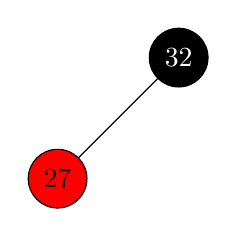
\begin{tikzpicture}[
		every node/.append style={circle, draw, minimum width=2em}
		,level/.style={sibling distance=.5\linewidth/#1}
		,b/.style={fill=black, text=white}
		,r/.style={fill=red}
		,baseline=(A.north)
	]
		\node [b] (A) {32}
			child {
				node [r, below left=of A] (B) {27}
			}
		;
	\end{tikzpicture}

	\item[Inserting 20]
	is done as the left child of 27 but we cannot color it red because 27 is already red and we also cannot color it black because $32 \rightarrow nil$ has a smaller black height than $32 \rightarrow 27 \rightarrow 20 \rightarrow nil$. We color it red and fix the tree with a right rotation.

	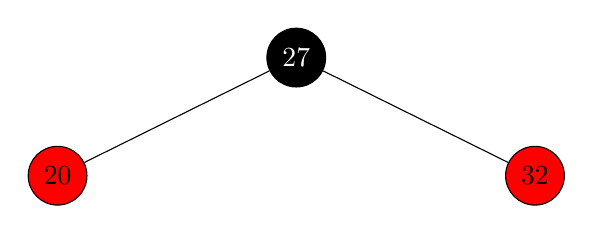
\begin{tikzpicture}[
		every node/.append style={circle, draw, minimum width=2em}
		,level/.style={sibling distance=.5\linewidth/#1}
		,b/.style={fill=black, text=white}
		,r/.style={fill=red}
		,baseline=(A.north)
	]
		\node [b] (A) {27}
			child {
				node [r] (B) {20}
			}
			child {
				node [r] (C) {32}
			}
		;
	\end{tikzpicture}

	\item[Inserting 15]
	as the left child of 20. We cannot color it red because its parent 27 is red and we cannot color it black, because $27 \rightarrow 20 \rightarrow 15 \rightarrow nil$ has a higher black height than $27 \rightarrow 32 \rightarrow nil$. We color the node red and fix the tree (case 1 and case 0).

	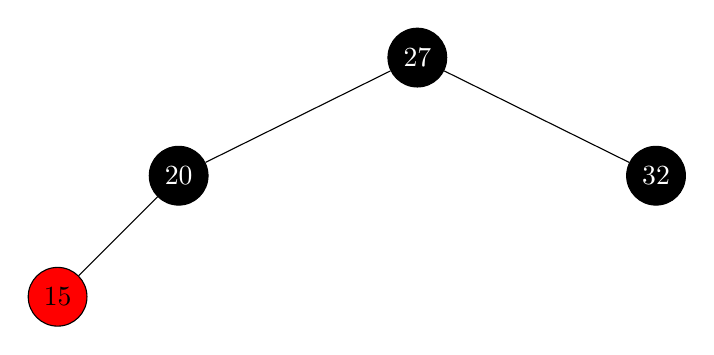
\begin{tikzpicture}[
		every node/.append style={circle, draw, minimum width=2em}
		,level/.style={sibling distance=.5\linewidth/#1}
		,b/.style={fill=black, text=white}
		,r/.style={fill=red}
		,baseline=(A.north)
	]
		\node [b] (A) {27}
			child {
				node [b] (B) {20}
				child {
					node [r, below left=of B] (D) {15}
				}
			}
			child {
				node [b] (C) {32}
			}
		;
	\end{tikzpicture}

	\item[Inserting 19]
	as the right child of 19. We cannot color it red because its parent 15 is already red and we cannot color it black because $27 \rightarrow 20 \rightarrow 15 \rightarrow 19 \rightarrow nil$ has a heigher black height than $27 \rightarrow 32 \rightarrow nil$ so we color it red and fix the tree.

	\begin{enumerate}
		\item 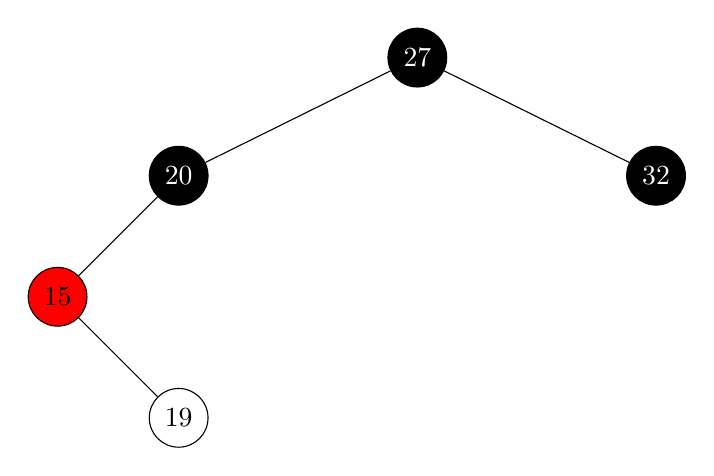
\begin{tikzpicture}[
			every node/.append style={circle, draw, minimum width=2em}
			,level/.style={sibling distance=.5\linewidth/#1}
			,b/.style={fill=black, text=white}
			,r/.style={fill=red}
			,baseline=(A.north)
		]
			\node [b] (A) {27}
				child {
					node [b] (B) {20}
					child {
						node [r, below left=of B] (D) {15}
						child {
							node [below right=of D] (E) {19}
						}
					}
				}
				child {
					node [b] (C) {32}
				}
			;
		\end{tikzpicture}
		\item 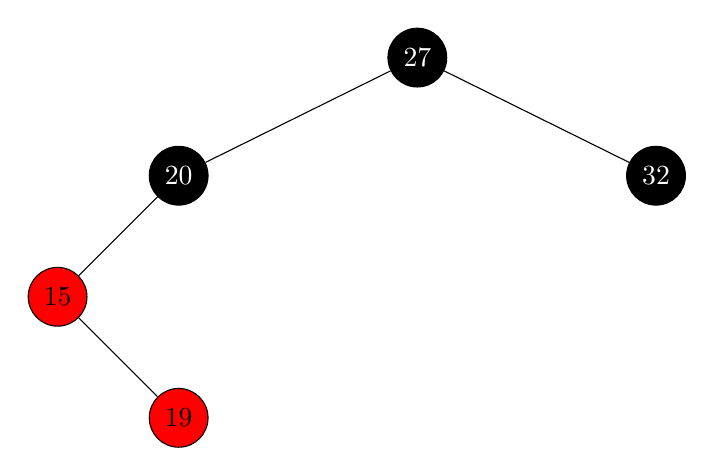
\begin{tikzpicture}[
			every node/.append style={circle, draw, minimum width=2em}
			,level/.style={sibling distance=.5\linewidth/#1}
			,b/.style={fill=black, text=white}
			,r/.style={fill=red}
			,baseline=(A.north)
		]
			\node [b] (A) {27}
				child {
					node [b] (B) {20}
					child {
						node [r, below left=of B] (D) {15}
						child {
							node [r, below right=of D] (E) {19}
						}
					}
				}
				child {
					node [b] (C) {32}
				}
			;
		\end{tikzpicture}\\
		(Case 2)
		\item 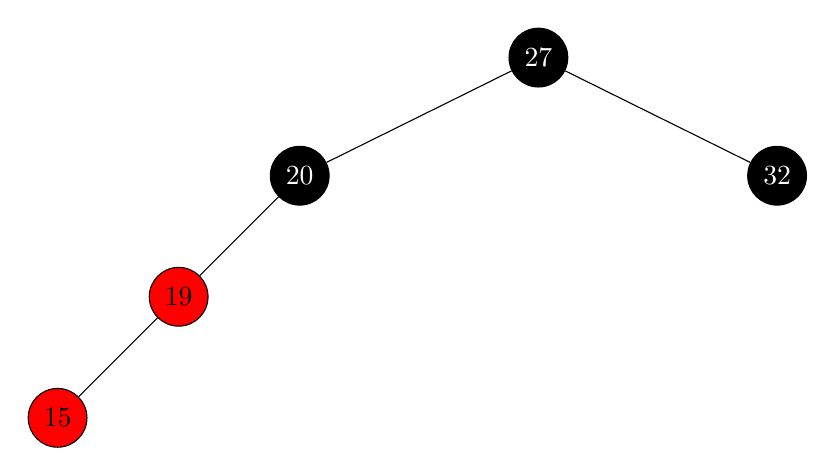
\begin{tikzpicture}[
			every node/.append style={circle, draw, minimum width=2em}
			,level/.style={sibling distance=.5\linewidth/#1}
			,b/.style={fill=black, text=white}
			,r/.style={fill=red}
			,baseline=(A.north)
		]
			\node [b] (A) {27}
				child {
					node [b] (B) {20}
					child {
						node [r, below left=of B] (D) {19}
						child {
							node [r, below left=of D] (E) {15}
						}
					}
				}
				child {
					node [b] (C) {32}
				}
			;
		\end{tikzpicture}\\
		(Case 3 step 1)
		\item 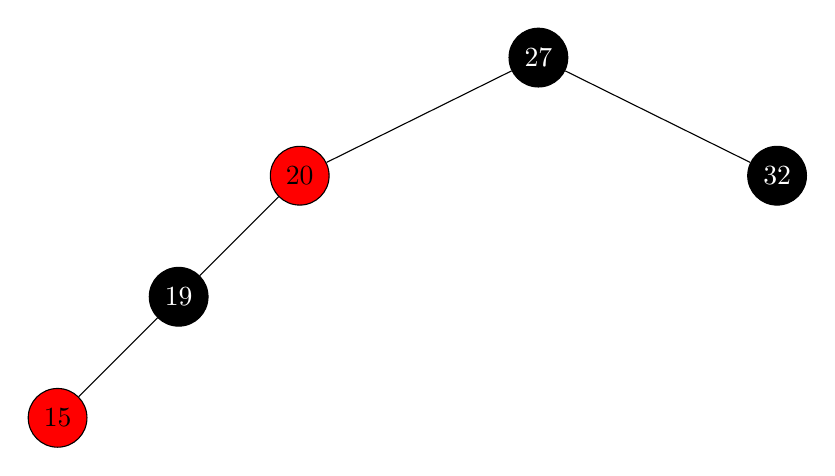
\begin{tikzpicture}[
			every node/.append style={circle, draw, minimum width=2em}
			,level/.style={sibling distance=.5\linewidth/#1}
			,b/.style={fill=black, text=white}
			,r/.style={fill=red}
			,baseline=(A.north)
		]
			\node [b] (A) {27}
				child {
					node [r] (B) {20}
					child {
						node [b, below left=of B] (D) {19}
						child {
							node [r, below left=of D] (E) {15}
						}
					}
				}
				child {
					node [b] (C) {32}
				}
			;
		\end{tikzpicture}\\
		(Case 3 step 2)
		\item 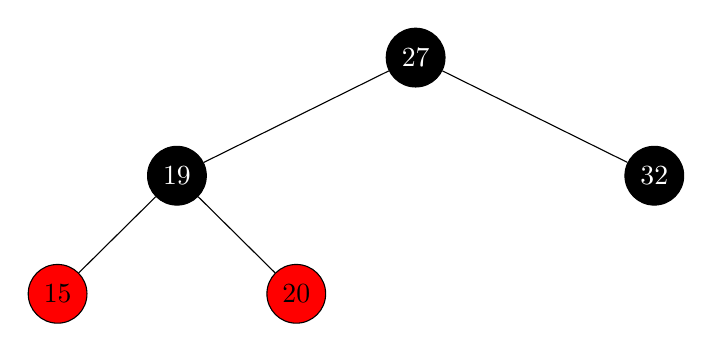
\begin{tikzpicture}[
			every node/.append style={circle, draw, minimum width=2em}
			,level/.style={sibling distance=.5\linewidth/#1}
			,b/.style={fill=black, text=white}
			,r/.style={fill=red}
			,baseline=(A.north)
		]
			\node [b] (A) {27}
				child {
					node [b] (B) {19}
					child {
						node [r] (D) {15}
					}
					child {
						node [r] (E) {20}
					}
				}
				child {
					node [b] (C) {32}
				}
			;
		\end{tikzpicture}
	\end{enumerate}

	\item[Inserting 33]
	as the right child of 32. We can cimply color it red without violating any property.
	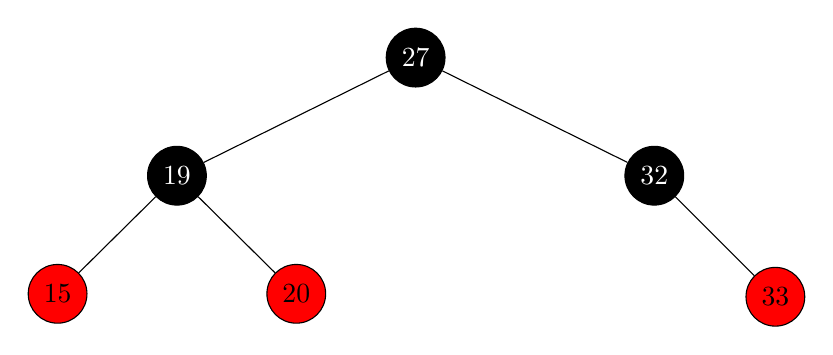
\begin{tikzpicture}[
		every node/.append style={circle, draw, minimum width=2em}
		,level/.style={sibling distance=.5\linewidth/#1}
		,b/.style={fill=black, text=white}
		,r/.style={fill=red}
		,baseline=(A.north)
	]
		\node [b] (A) {27}
			child {
				node [b] (B) {19}
				child {
					node [r] (D) {15}
				}
				child {
					node [r] (E) {20}
				}
			}
			child {
				node [b] (C) {32}
				child {
					node [r, below right=of C] (F) {33}
				}
			}
		;
	\end{tikzpicture}

	\item[Deleting 19]
	\item[Deleting 32]
\end{description}

\section{} %4

You do not actually need parent pointers to traverse back up the tree because you begin by going down the tree and at this stage you can save the path you took to get to where you currently are. This could be done, for example, by using a recursive insertion function which would keep track of the path in the stack frames. Alternatively you could have an iterative traversal function and store a list containing all the nodes in the path to where we are now. This would be more efficient but also more complicated.

In the recursive approach we would just fix the problem at the current node, then return, which gets us one level higher where we can proceed doing the same until we return from the oldest stack (that which contains the root node) frame and are done.

The drawback of the recursive approach would be that you would have a lot of duplication because in each stack frame you would need to store more than one node because fixing one level requires some insight into the levels above. Many of the stack frames would contain overlapping information.

\section{} %5

\end{document}
